\documentclass{beamer}[10]
% preamble speciale Jacob Harder
% 31. jan. 2020

%packages

\usepackage[utf8]{inputenc} %utf8 is probably good
\usepackage{amsmath}
\usepackage{amssymb}
\usepackage{amsthm}
\usepackage{graphicx} %for including images
\usepackage{float} %for exact placement of figure (and more?)
\usepackage{mathtools} %for \mathclap (stacking under sums)
\usepackage{dsfont} %for boldface numbers
\usepackage{bm} %vectors in bold
\usepackage[ruled,vlined]{algorithm2e}
\usepackage{cleveref}
\usepackage{ifthen}
\usepackage{commath}
\usepackage[a4paper,width=150mm,top=25mm,bottom=25mm]{geometry}
\usepackage{upgreek}
%\usepackage[inline]{enumitem}
\usepackage{multicol}
%\usepackage{fancyhdr} %maybe later..
%\pagestyle{fancy}
\usepackage{mathabx}
\usepackage{csquotes}
\usepackage{tikz}
\usepackage{outline} %for subitems in lists

%front page
\usepackage{wallpaper}
\usepackage{titling}

%bibliography
\usepackage[numbers]{natbib}
\bibliographystyle{plainnat}
\newcommand{\mcite}[1]{[\citenum{#1}, \citeauthor{#1} (\citeyear{#1})]}
\newcommand{\ncite}[1]{\cite{#1}}

%linespread and geometry
\linespread{1.3}

%commands
\newcommand{\Cal}{\mathcal}
\newcommand{\cl}{\mathcal}
\newcommand{\fk}{\mathfrak}
\newcommand{\bb}{\mathbb}
\newcommand{\Q}{\bb{Q}}
\newcommand{\Z}{\bb{Z}}
\newcommand{\N}{\bb{N}}
\newcommand{\R}{\bb{R}}
\newcommand{\C}{\bb{C}}
\newcommand{\E}{\bb{E}}
\newcommand{\Rext}{\ol{\ul{\R}}}
\newcommand{\Var}{\mathrm{Var}}
\newcommand{\Prob}{\mathds{P}} %fundamental probability measure
\newcommand{\idc}{\mathds{1}}
\newcommand{\ve}{\varepsilon} %abbreviation for epsilon
\newcommand{\Yp}{\Upupsilon} %abbreviation for Ypsilon
\newcommand{\difd}{\; \mathrm{d}} %differential d
\newcommand{\wt}{\widetilde}
\newcommand{\wh}{\widehat}
\newcommand{\ol}{\overline}
\newcommand{\ul}{\underline}
\newcommand{\Mid}{\;\middle\vert\;}
\newcommand{\id}{\text{id}}
\newcommand{\supp}{\text{supp}}
\newcommand{\defemph}[1]{\textbf{#1}} %first-mentions of names
\DeclarePairedDelimiter\ceil{\lceil}{\rceil}
\DeclarePairedDelimiter\floor{\lfloor}{\rfloor}
\DeclareMathOperator*{\argmax}{argmax}
\DeclareMathOperator*{\argmin}{argmin}
\newcommand{\defeq}{\vcentcolon=} %definition equality symbol
%add single eq. tag in align*
\newcommand\numberthis{\addtocounter{equation}{1}\tag{\theequation}}
\newcommand{\rleft}[1]{\rotatebox[origin=c]{90}{\ensuremath{#1}}}
\newcommand{\vrel}[3]{ % for vertical subseteq e.g.
\vcenter{\halign{\hfill##\hfill\cr
\ensuremath{#1}\cr
\rotatebox[origin=c]{270}{\ensuremath{#2}}\cr
\ensuremath{#3}\cr
}}}
\newcommand{\lar}{\leftrightarrow}
\newcommand{\Span}{\mathrm{span}}
\newcommand{\Gr}{\mathrm{Gr}}

%theorems
\theoremstyle{definition}
\newtheorem{thm}{Theorem}[chapter]
\newtheorem{lem}[thm]{Lemma}
\newtheorem{defn}[thm]{Definition}
\newtheorem{cor}[thm]{Corollary}
\newtheorem{rem}[thm]{Remark}
\newtheorem{prop}[thm]{Proposition}
\newtheorem{asm}{Assumption}
\newtheorem{example}[thm]{Example}
%\newtheorem{cond}{Condition}
\newtheorem{sett}{Setting}
\newtheorem{innercond}{Condition}
\newenvironment{cond}[1]
  {\renewcommand\theinnercond{#1}\innercond}
  {\endinnercond}

%cref
\crefname{algocf}{alg.}{algs.}
\Crefname{algocf}{Algorithm}{Algorithms}
\crefname{innercond}{}{}
\Crefname{innercond}{}{}


\usepackage{pgf}
%\usepackage[danish]{babel}
\usepackage[utf8]{inputenc}
\usepackage{beamerthemesplit}
\usepackage{graphics,epsfig, subfigure}
\usepackage{url}
\usepackage{srcltx}
\usepackage{hyperref}
\usepackage{tikz-dependency}
\usepackage{tikz-qtree}
\usepackage{wrapfig}
\usepackage{algorithm2e}
\usepackage{algorithmic}

\definecolor{kugreen}{RGB}{50,93,61}
\definecolor{kugreenlys}{RGB}{132,158,139}
\definecolor{kugreenlyslys}{RGB}{173,190,177}
\definecolor{kugreenlyslyslys}{RGB}{214,223,216}
\setbeamercovered{transparent}
\mode<presentation>
\usetheme[width=1.6cm,numbers,totalnumber,compress,sidebarshades]{PaloAlto}
\setbeamertemplate{footline}[frame number]

\usecolortheme[named=kugreen]{structure}
\useinnertheme{circles}
\usefonttheme[onlymath]{serif}
\setbeamercovered{transparent}
\setbeamertemplate{blocks}[rounded][shadow=true]

\logo{\includegraphics[width=0.5cm]{KULogo}}

\makeatletter
\beamer@headheight=1.5\baselineskip     %controls the height of the headline, default is 2.5
\makeatother

\title{Theoretical aspects of Q-learning}
\subtitle{Masters thesis defense}
\institute{Jacob Harder \\
Department of Mathematical Sciences \\ University of Copenhagen}
\date{26 June, 2020}

\begin{document}

\frame{\titlepage \vspace{-0.5cm}
}

\frame
{
\frametitle{Overview}
\tableofcontents%[pausesection]
}

\section{Introduction}

\begin{frame}
  \frametitle{Q-learning as AI}
  \usetikzlibrary{trees, arrows, shapes.multipart}
  \tikzset{
    edge from parent/.style={draw,-latex},
    level distance=1.5cm
  }
  \begin{tikzpicture}[
      every node/.style={align=center,anchor=north},
    ]
    \Tree [.{Artificial Intelligence (AI)}
      [.{Machine Learning (ML)}
	[.{Reinforcement Learning (RL)}
	  [.{\defemph{Q-learning}} ]
	]
	[.{Supervised Learning, etc.} ]
      ]
    ]
  \end{tikzpicture}
\end{frame}

\frame{
  \frametitle{Machine learning}
  Machine Learning is
  ``the study of computer algorithms that improve automatically through
  \emph{experience}''.
  \begingroup
  \fontsize{10pt}{12pt}\selectfont
  \begin{itemize}
    \item[-] \defemph{Supervised learning}: Tasks are learned from data 
      based on feedback from a
      \emph{supervisor}. E.g. image classification.
    \item[-] \defemph{Unsupervised learning}:
      Data is given without evaluatory feedback,
      general trends about the data are analysed.
      E.g. principal component analysis, and cluster analysis.
    \item[-] $\rightarrow$\footnote{``$\rightarrow$'': Our main area of focus
      in this thesis.}
	\defemph{Reinforcement learning}: Algorithms
      which learns through interactions with an \emph{environment}.
  \end{itemize}
  \endgroup
}

\frame{
  \frametitle{Challenges in RL}
  Challenges in Reinforcement Learning include:
  \begingroup
  \fontsize{10pt}{12pt}\selectfont
  \begin{itemize}
    \item[-] \defemph{Exploration-exploitation trade-off}. Training and
      performing occurs simultaneously so one optimizes the total reward on some
      time horizon. This is studied
      in e.g. the multi-armed bandit problem.
    \item[-] $\rightarrow$ \defemph{Deriving optimal policies}.
      Training and performing is
      distinguished and emphasis is put on the expected performance of the final
      derived policy rather than rewards occuring during training.
  \end{itemize}
  \endgroup
}

\subsection{The environment}

\frame{
  \frametitle{The environment}
  The \defemph{environment} in RL is often formalized as a
  \defemph{Markov decision process} (MDP), which consists of
  \begin{itemize}
    \item[-] $\Cal{S}$ a 
      measurable space of states.
    \item[-] $\Cal{A}$ a 
      measurable space of actions.
    \item[-] $P : \Cal{S} \times \Cal{A} \leadsto \Cal{S}$
      a transition kernel\footnote{
	Here $\leadsto$ denotes a \emph{stochastic mapping} (to be
      defined soon).}.
    \item[-] $R : \Cal{S} \times \Cal{A} \leadsto \R$
      a reward kernel discounted by
    \item[-] a discount factor $\gamma \in [0,1)$.
    \item[-] $\frak{A}(s) \subseteq \cl{A}$ a set of admissable actions
      for each $s \in \cl{S}$.
  \end{itemize}
}

\frame{
  \frametitle{Examples of MDPs}
  Examples of Markov decision processes include
  \begin{itemize}
    \item[-] Board games where one plays against a fixed opponent,
      e.g. \emph{chess} where the set of states $\cl{S}$
      is the set of all obtainable chess-positions.
    \item[-] Time-descretized physics simulations with action inputs and reward
      outputs, including most single player video games and
      the classic \emph{cartpole} example (balancing a stick).
  \end{itemize}
}

\frame{
  \begingroup
  \fontsize{10pt}{12pt}\selectfont
  \frametitle{The probability kernels}
  \begin{block}{Probability kernel}
    A \defemph{probability kernel}
    (also called a \emph{stochastic mapping}, \emph{stochastic kernel}
    or \emph{Markov kernel})
    $\kappa : \cl{X} \leadsto \cl{Y}$ is a collection of probability measures
    $\kappa(\cdot \mid x)$, one for each $x \in \cl{X}$ such that
    for any measurable set $B \subseteq \cl{Y}$ the function
    $x \mapsto \kappa(B \mid x)$ is measurable.
  \end{block}
  The transition probability measure $P(\cdot \mid s, a)$ 
  of the pair $(s, a) \in \cl{S} \times \cl{A}$ determines
  what states are likely to follow after \emph{being} in state $s$ and
  \emph{choosing} action $a$. Similarly from the reward kernel $R$ one obtains the
  measure $R(\cdot \mid s, a)$ determining the reward distribution following
  the timestep $(s, a)$.
  \endgroup
}

\frame{
  \frametitle{Policies}
  Given a Markov decision process one can define a \defemph{policy} $\pi$ by
  sequence of probability kernels $\pi = (\pi_1, \pi_2, \dots)$ where
  $\pi_i : \cl{H}_i \leadsto \cl{A}$ and
  $\cl{H}_i = \cl{S} \times \cl{A} \times \dots \times \cl{S}$
  is the \emph{history space} at the $i$th timestep.
}

\frame{
  \frametitle{Stochastic processes}
  An MDP $(\cl{S}, \cl{A}, P, R, \gamma)$ together with a policy
  $\pi = (\pi_1, \pi_2, \dots)$ and a distribution $\mu$ on $\cl{S}$
  give rise to a stochastic process
  $(S_1, A_1, S_2, A_2, \dots) \sim \kappa_\pi \mu$ such that for any
  $i \in \N$ we have
  $(S_1, A_1, \dots, S_i) \sim P\pi_{i-1} \dots P \pi_1 \mu$
  where $P\pi_{i-1} \dots P \pi_1$ denotes the \emph{kernel-composition}
  of the probability kernels $P, \pi_1, \dots, \pi_{i-1}$.
  We denote by $\E_s^\pi$ expectation over $\kappa_\pi \mu$ where
  $\mu = \delta_s$, that is, $S_1 = s$ a.s.
}

\subsection{Value functions and the goal of RL}

\frame{
  \frametitle{Policy evaluation}
  For a policy $\pi$ we can define the policy evaluation function:
  \begin{block}{Policy evaluation}
    \begingroup
    \small
    Denote by $r(s, a) = \int x \difd R(x \mid s, a)$ the \emph{expected
    reward function}. We define the \defemph{policy evaluation function} by
    $$ V_\pi(s) = \E_s^\pi \sum_{i=1}^\infty \gamma^{i-1} r \circ \rho_i $$
    where $\rho_i$ is projection onto $(\cl{S}_i, \cl{A}_i)$.
    \endgroup
  \end{block}
  This an example of a (state-) \emph{value function}, as it assigns a real
  number to every state $s \in \cl{S}$.
}

\frame{
  \frametitle{Finite policy evaluation}
  Similar to the infinite horizon policy evaluation we can also consider
  a finite horizon version:
  \begin{block}{Definition: Finite policy evaluation}
    We define the function $V_{n, \pi} : \cl{S} \to \R$ by
    \[ V_{n,\pi}(s) = \E_{s}^\pi \sum_{i=1}^n \gamma^{i-1} r \circ \rho_i \]
    called the $k$th \defemph{finite policy evaluation}\footnote{When
    $n=0$ we say $V_{0,\pi} = V_0 \defeq 0$ for any $\pi$.}.
  \end{block}
}

\frame{
  \frametitle{Optimal value function}
  \begingroup
  \footnotesize
  \begin{block}{Definition: Optimal value functions}
    \begin{align*}
      V_n^*(s) \defeq & \; \sup_{\pi \in R\Pi} V_{n,\pi}(s)
      = \sup_{\pi \in R\Pi} \E_s^\pi \sum_{i=1}^n r_i
      \\
      V^*(s) \defeq & \; \sup_{\pi \in R\Pi} V_\pi(s)
      = \sup_{\pi \in R\Pi} \E_s^\pi \sum_{i=1}^\infty r_i
    \end{align*}
    This is called the \defemph{optimal value function} (and the $n$th
    optimal value function).
    A policy $\pi^* \in R\Pi$ for which $V_{\pi^*} = V^*$ is called an
    \defemph{optimal policy}.
    If $V_{n, \pi^*} = V^*_n$ then $\pi^*$ is called $n$-optimal.
  \end{block}
  Provided such an optimal policy $\pi^*$ exists,
  obtaining such a policy is the ultimate goal
  of Reinforcement Learning.
  \endgroup
}

\subsection{Value iteration}

\frame{
  \frametitle{Greediness}
  In order to show existence of optimal policies and talk about algorithms
  which can determine such policies, we define the concept of \emph{greediness}.
}

\frame{
  \frametitle{Greedy actions}
  \begingroup
  \footnotesize
  The purpose of (most) value functions $V : \cl{S} \to \R$ is to give an estimate
  on how \emph{good} a certain state is, in terms of the rewards one may expect
  after visiting it.
  \\ This give rise to the idea of \emph{greedy actions}, that is,
  actions leading to states high \emph{values} (according to $V$).
  \begin{block}{Definition greedy actions}
    Let $V : \cl{S} \to \R$ be a measurable value-function.
    We define
    \[ G_V(s) = \argmax_{a \in \frak{A}(s)} T_a V(s) \subseteq \frak{A}(s) \]
    as the set of \defemph{greedy} actions w.r.t. $V$.
  \end{block}
  \endgroup
}

\frame{
  \frametitle{Greedy policies}
  Greedy actions leads to \emph{greedy policies}:
  \begin{block}{Definition: Greedy policy}
    Let $V : \cl{S} \to \R$ be a measurable value-function and
    let $\tau : \cl{S} \leadsto \cl{A} \in S\Pi$ be a stationary policy.
    If there exists a measurable $G_V^\tau(s) \subseteq G_V(s)$
    such that
    \[ \tau(G_V^\tau(s) \mid s) = 1 \]
    for every $s \in \cl{S}$, then $\tau$ is called greedy w.r.t. $V$.
    We will often denote a $V$-greedy policy by $\tau_V$.
  \end{block}
}

\frame{
  \frametitle{Existence of greedy policies}
  \begingroup
  \footnotesize
  \begin{block}{Theorem (Existence of greedy policies)}
    Suppose $V: \cl{S} \to \R$ is \emph{upper semicontinuous} and that
    \begin{itemize}
      \item[1.] $\cl{S}$ and $\cl{A}$ are standard Borel.
      \item[2.]  The set of admissable actions 
	$\frak{A}(s) \subseteq \cl{A}$ is compact for all $s \in \cl{S}$
	and $\Gamma = \{ (s, a) \in \cl{S} \times \cl{A} \mid a \in \frak{A}(s) \}$
	is a closed subset of $\cl{S} \times \cl{A}$.
      \item[3.] The transition kernel $P$ is continuous.
      \item[4.] The expected reward function $r = \int r' \difd R(r' \mid \cdot)$
	is upper semicontinuous and bounded from above.
    \end{itemize}
    Then there exists a deterministic policy $\pi_V$ which is greedy for $V$.
  \end{block}
  If assumptions 1.-4. hold we will say that the MDP is \emph{greedy}.
  \endgroup
}

\frame{
  \frametitle{Policy iteration}
  \begingroup
  \footnotesize
  Using the concepts we have defined one can get the following idea:
  Iteratively generate value functions by
  picking greedy policies and then evaluating these policies.
  This is called \emph{policy iteration}.
  \begin{figure}
    \centering
    \begin{tikzpicture}
      \def \n {3}
      \def \radius {1cm}
      \def \margin {30} % margin in angles, depends on the radius
      \def \txt {
	{$V$},
	{$\tau_V$},
	{$V_{\tau_V}$}
      }

      \foreach \t [count=\s from 0] in \txt
      {
	\node[draw, circle] at ({360/\n * (\s - 1)}:\radius) {\t};
	\draw[->, >=latex] ({360/\n * (\s - 1)+\margin}:\radius)
	arc ({360/\n * (\s - 1)+\margin}:{360/\n * (\s)-\margin}:\radius);
      }
    \end{tikzpicture}
  \end{figure}
  Policy iteration is a well studied algorithm and can be shown to
  converges to optimum for a variety of environments. We will however
  move on to talk about a related concept called
  \emph{value iteration}.
  \endgroup
}

\frame{
  \frametitle{Operators on value functions}
  Before defining value iteration we introduce some operators
  \begin{block}{The $T$-operators}
    For a stationary policy $\tau \in S\Pi$ and a value function
    $V:\Cal{S} \to \R \in \cl{L}_\infty(\cl{S})$
    we define the operators 
    \begin{gather*}
      \text{The policy evaluation operator: }
      \\ T_\tau V \defeq s \mapsto \int r(s, a)
      + \gamma V(s') \difd (P \tau)(a, s'\mid s)
      \\ \text{The Bellman optimality operator: }
      \\ T V \defeq s \mapsto 
      \sup_{a \in \frak{A}(s)} \left(r(s, a) + \gamma \int V(s')
      \difd P(s' \mid s, a) \right)
    \end{gather*}
  \end{block}
}

\frame{
  \frametitle{Properties of the $T$-operators}
  \begingroup
  \footnotesize
  \begin{block}{Proposition (Properties of the $T$-operators)}
    \begin{itemize}
      \item $V_{k, \pi} = T_{\tau_1} V_{k-1, (\tau_2, \dots)}
	= T_{\tau_1} \dots T_{\tau_k} V_0$.
      \item $V_\pi = \lim_{k \to \infty} T_{\tau_1} \dots T_{\tau_k} V_0$
      \item For the stationary policy $\tau$ we have $T_\tau V_\tau = V_\tau$.
      \item $T$ and $T_\tau$ are $\gamma$-contractive
	on $\Cal{L}_\infty(\Cal{S})$.
      \item $V_\tau$ is the unique bounded fixed point of $T_\tau$
	in $\Cal{L}_\infty(\Cal{S})$.
    \end{itemize}
  \end{block}
  This way $T_\tau$ can be interpreted as a 'one-step policy evaluation'.
  On the other hand $T$ can be interpreted as a 'one-step evaluation, when
  always choosing greedy actions'.
  \endgroup
}

\frame{
  \frametitle{Value iteration}
  \begingroup
  \footnotesize
  \emph{Value iteration} is the iterative application of the $T$-operator.
  The following theorem show why
  value iteration is a 
  central idea Reinforcement Learning\footnote{Actually value iteration
  is inherited from dynamic programming.}.
  \begin{block}{Theorem (Existence optimal policies
    \& convergence of value iteration)}
    Given a greedy MDP we have that
    \[ V^*_k = T^k V_0 = T_{\tau^*_{k-1}} \dots T_{\tau^*_0} V_0
    = V_{k, (\tau^*_{k-1}, \dots, \tau^*_0)} \]
    The policy $(\tau^*_{k-1}, \dots, \tau^*_0)$ is a deterministic
    $k$-optimal policy
    where $\tau_k^* = \tau_{T^k V_0}$ is any deterministic
    greedy policy for $T^k V_0$ for any $k \in \N$.
    \\ Furthermore $V^* = \lim_{k\to\infty} T^k V^*_0$, the greedy policy
    $\tau^* = \tau_{V^*}$ exists and an optimal policy.
  \end{block}
  \endgroup
}

\frame{
  \frametitle{Convergence rates}
  We can also show that the optimal value function $V^*$ is a fixed point of
  the Bellman optimality operator $T$.
  \[ TV^* = V^* \]
  This is often called \emph{Bellman's optimality equation}.
  \\ Recalling that $T$ is $\gamma$-contractive, by Banach's fixed point theorem 
  we get exponential convergence rates for value iteration:
  \[ \norm{T^k V - V^*} \leq \gamma^k \norm{V - V^*}_\infty = \cl{O}(\gamma^k) \]
}

\frame{
  \frametitle{Example: Gridworld}
  \begingroup
  \footnotesize
  \begin{wrapfigure}{R}{0.5\textwidth}
    \centering
    \begin{tikzpicture}
      \draw[step=0.5cm, color=gray] (0,0) grid (2.5,2.5);
      \node (A) at (0.75,2.25) {A};
      \node (A') at (0.75,0.25) {A'};
      \node (B) at (1.75,2.25) {B};
      \node (B') at (1.75,1.25) {B'};
      \draw [->][bend left=15] (A) edge node[left] {\scriptsize{+10}} (A');
      \draw [->][bend left=15] (B) edge node[left] {\scriptsize{+5}} (B');
    \end{tikzpicture}
  \end{wrapfigure}
  The \emph{gridworld} MDP consist of 25 states $\cl{S} = [5]^2$ and 4 actions
  $\cl{A} = \{U, D, L, R\}$ for \emph{up}, \emph{down}, \emph{left} and 
  \emph{right} and moves the agent
  1 square up, down, left or right.
  A reward of 0 is given by default, except when
  \begingroup
  \scriptsize
  \begin{itemize}
    \item[-] \emph{hitting the boundary} a reward of -1 is given
    \item[-] when in $A = (2,1)$ any action moves to $A' = (2,5)$ and
      is rewarded 10.
    \item[-] when in $B = (4,1)$ any action moves to $B' = (4,3)$ and
      is rewarded 5.
  \end{itemize}
  \endgroup
  Finally $\gamma = 0.9$ is the standard value of the discount factor
  in this example.
  \endgroup
}

\frame{
  \frametitle{Example: Gridworld}
  \begin{figure}
    \centering
    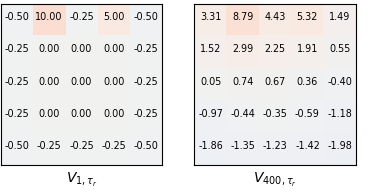
\includegraphics[scale=0.8]{figs/gridworld1_1.png}
    \caption{Policy evaluations of the gridworld environment.
      Note that $V_{\max} \cdot \gamma^{400} = 100 \cdot (0.9)^{400}
      \approx 4.97 \cdot 10^{-17}$ so $V_{\tau_r, 400}$
      are very close to the true infinite horizon value functions
    $V_{\tau_r}$ (providing numerical errors are insignificant).}
    \label{fig:gw1}
  \end{figure}
}

\frame{
  \frametitle{Example: Gridworld}
  \begin{figure}
    \centering
    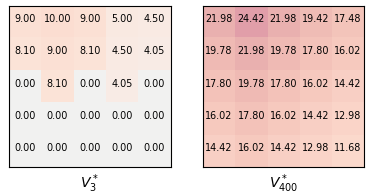
\includegraphics[scale=0.8]{figs/gridworld1_2.png}
    \caption{Optimal value functions of the gridworld environment.
      By the same upper bound as before we have
    $\norm{V^* - V^*_{400}}_\infty < 4.97 \cdot 10^{-17}$.}
    \label{fig:gw1}
  \end{figure}
}

\frame{
  \frametitle{Example: Gridworld}
  \vspace{-0.35cm}
  \begin{figure}
    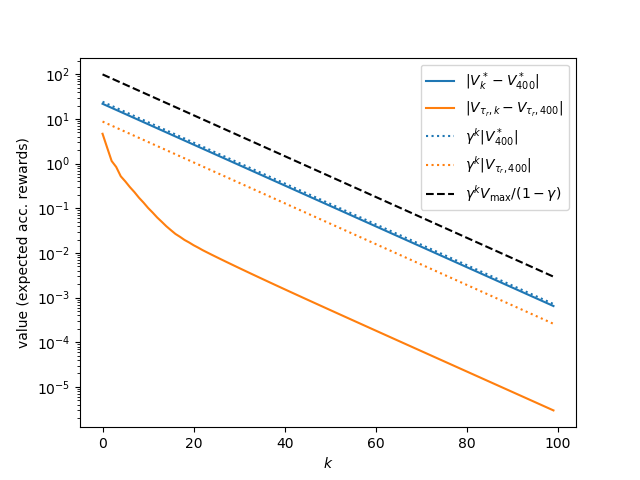
\includegraphics[scale=0.45]{figs/gridworld2.png}
  \end{figure}
  \footnotesize Convergence of gridworld value functions compared with
  the theoretical bounds. The black dashed line is the general theoretical
  bound for both $T$ and $T_{\tau}$ by Banachs fixed point theorem and
  the maximum value $V_{\max} = R_{\max} / (1-\gamma)$.
  The dotted blue and orange uses $\abs{V_k^*}$ and $\abs{V_{\tau, k}}$ 
  respectively, which might not be available.
  ($\gamma = 0.9$).
}

\subsection{Q-functions}

\frame{
  \frametitle{Q-functions}
  A \defemph{Q-function}
  is simply any function assigning a real number to every state-action pair.
  They are also called (state-) \emph{action value functions}.
  \\ \vspace{0.3cm}
  A \defemph{Q-learning} algorithm is any algorithm which uses Q-functions
  to derive a policy for an environment\footnote{Some authors refer to
    Q-learning as a specific variation of temporal difference learning,
    but this fails to capture many algorithms which are also referred to
  as \emph{Q-learning algorithms}.}.
}

\frame{
  \frametitle{Motivation for Q-functions}
  A clear advantage of working with Q-function
  $Q:\Cal{S}\times\Cal{A} \to \R$ rather than a value function
  $V:\Cal{S}\to \R$,
  is that finding the optimal action $a^* \in \frak{A}(s)$ at state $s$
  requires only a maximization over the Q-function itself:
  $a^* = \argmax_{a \in \frak{A}(s)} Q(s,a)$.
  This should be compared to finding an optimal action
  according to a value function $V$:
  $a^* = \argmax_{a \in \frak{A}(s)} r(s,a) + \gamma \E_{P(\cdot \mid s,a)} V$.
}

\frame{
  \frametitle{Greed with Q-functions}
  Formally we define greedy actions and policies w.r.t. a Q-function as
  \begingroup
  \small
    Let $Q:\cl{S} \times \cl{A} \to \R$ be a measurable Q-function and
    $\tau: \cl{S} \leadsto \cl{A}$ be a (stationary) policy.
  \begin{block}{Greedy policy}
    Define the set of
    \emph{greedy actions} by
    $G_Q(s) \defeq \argmax_{a \in \frak{A}(s)} Q(s, a)$.
    If there exist a measurable set $G_Q^\tau(s) \subseteq G_Q(s)$
    for every $s \in \Cal{S}$ such that
    \[ \tau \left( G_Q^\tau(s) \Mid s \right) = 1 \]
    then $\tau$ is said to be \defemph{greedy} with respect to $Q$ and is
    denoted $\tau_Q$.
  \end{block}
  \endgroup
}

\frame{
  \frametitle{Q-function operators}
  \begingroup
  \footnotesize
  Moreover we define $T$-operators similar to ones for value functions
  \begin{block}{Operators for Q-functions}
    For any stationary policy $\tau \in S\Pi$ and
    integrable Q-function $Q:\Cal{S} \times \Cal{A} \to \R
    \in \cl{L}_\infty(\cl{S} \times \cl{A})$ we define
    \begin{gather*}
      \text{Next-step operator: }
      \\ P_\tau Q(s, a) = \int Q(s', a') \difd \tau P(s', a' \mid s, a)
      \\ \text{Policy evaluation operator: } 
      \\
      T_\tau Q(s, a) = 
      r(s, a) + \gamma \int Q(s', a') \difd \tau P(s', a' \mid s, a)
      \\ \text{Bellman optimality operator: } 
      \\ T Q(s, a) = r(s, a) + \gamma
      \int \max_{a' \in \Cal{A}} Q(s', a') \difd P(s' \mid s, a)
    \end{gather*}
    where $T_a = T_{\delta_a}$.
  \end{block}
  \endgroup
}

\frame{
  \frametitle{Relation between value- and Q-functions}
  \begingroup
  \footnotesize
  \begin{block}{Theorem (Relations between Q- and value functions)}
    Let $\pi = (\tau_1, \tau_2, \dots) \in M\Pi$ be a Markov policy
    and $\tau \in S\Pi$ stationary. Then
    \begin{itemize}
      \item[-] Policy evaluations are related by
	$\E_{\tau(\cdot \mid s)} Q_{k, \pi} = V_{k+1, (\tau, \pi)}(s)$.
      \item[-] $T_\tau$-operators are related by $T_\tau Q_{k, \pi}(s, a)
	= r + \gamma \E_{P(\cdot \mid s, a)} T_\tau V_{k, \pi}$.
      \item[-] $\tau$ is greedy for
	$Q_{k, \pi}$ if and only if $\tau$ is greedy for $V_{k, \pi}$
	and
	\\ $\tau$ is greedy for $Q_\pi$ if and only if $\tau$ is greedy for
	$V_\pi$.
      \item[-] Optimal policies are related by
	$\max_{a \in \frak{A}(s)} Q^*(s, a) = V^*(s)$ and
	\[ Q^*_k(s, a) = r(s, a) + \gamma \E_{P(\cdot \mid s, a)} V^*_k,
	\quad Q^*(s, a) = r(s, a) + \gamma \E_{P(\cdot \mid s, a)} V^* \]
    \end{itemize}
  \end{block}
  \endgroup
}

\frame{
  \frametitle{Properties of Q-functions}
  Because of the close relations
  many properties are inherited from value function to Q-functions:
  \begin{block}{Proposition (Properties of Q-functions)}
    Let $\pi = (\tau_1, \tau_2, \dots) \in M\Pi$ be a Markov policy
    and $\tau \in S\Pi$ stationary. Then
    \begin{itemize}
      \item $Q_{k, \pi} = T_{\tau_1} \dots T_{\tau_k} Q_0$ and
	$Q^*_k = T^k Q^*_0$.
      \item $Q_\pi = \lim_{k \to \infty} Q_{k, \pi}$ and
	$Q^* = \lim_{k\to\infty} Q_k^*$. 
      \item $T,\; T_\tau$ are $\gamma$-contractive on
	$\Cal{L}_\infty(\Cal{S}\times\Cal{A})$
	and $Q^*,\; Q_\tau$ are their unique fixed points.
      \item $Q^* = Q_{\tau^*}$
    \end{itemize}
  \end{block}
}

\subsection{Q-iteration}

\begin{frame}[fragile]
  \frametitle{Q-iteration}
  \begingroup
  \small
  \emph{Q-iteration} is the analogue of value-iteration for Q-function.
  It can be stated in the form of an algorithm as follows:
  \begin{block}{Algorithm (Q-iteration)}
    \begin{algorithm*}[H]
      \KwData{MDP $(\cl{S}, \cl{A}, P, R, \gamma)$, number of iterations $K$}
      Initialize expected reward function
      $r \leftarrow \int x \difd R(x \mid \cdot)$
      and $\wt{Q}_0 \leftarrow r$.
      \\ \For{$k = 0,1, \dots K-1$}{
	$\wt{Q}_{k+1} \leftarrow T \wt{Q}_k$
      }
      \KwOut{$\wt{Q}_K$}
    \end{algorithm*}
  \end{block}
  In the context of a greedy MDP we immedially have that the output of
  the Q-iteration algorithm $\wt{Q}_K = Q^*_K$ is $K$-optimal.
  \endgroup
\end{frame}

\frame{
  \frametitle{Value iteration with Q-functions}
  Similar to value-iteration we can use
  Banach fixed point theorem with the contractive properties
  of the $T$-operator for Q-functions to obtain exponential
  convergence of Q-iteration:
  \begin{block}{Proposition (Convergence of Q-iteration)}
    Suppose the Q-iteration algorithm is run with a greedy MDP.
    Then the output $\wt{Q}_K = Q^*_K$ satisfy
    \[ \norm{Q^* - Q^*_K}_\infty \leq \gamma^K V_{\max} \]
  \end{block}
}

\begin{frame}
  \frametitle{Why are we not done?}
  \begingroup
  \footnotesize
  We have exponential convergence for the broad class of problems expressible
  as a greedy MDP. This class includes highly difficult environments such as
  control problems in time-descretized simulation environments such as computer
  games, including the game of \emph{chess}. Are we then done?
  \begin{block}{Problems of Q-iteration}
    \begin{itemize}
      \item[1.] It is assumed that we know how to integrate over $P$ and $R$.
	\begin{itemize}
	  \item[-] The distributions of $P$ and $R$ might be impractical to
	    work with in a computer.
	  \item[-] It is common in RL to assume that $P$ and $R$ are unknown,
	    thus including a variety of environments, which we have not yet
	    considered.
	\end{itemize}
      \item[2.] It is assumed that we know how to represent $Q$ functions in 
	a feasible way in a computer.
    \end{itemize}
  \end{block}
  \endgroup
\end{frame}

\begin{frame}
  \frametitle{Example: Chess}
  The state space of chess is very large
  (roughly $\abs{\cl{S}_{\hrm{chess}}} \geq 10^{43}$).
  This means that if we were to use Q-iteration naively
  (with finite implementation as in the gridworld example)
  then we would have to store a vector of
  roughly $N \cdot 10^{43}$ real numbers for each Q-function we define,
  where $N$ is the average number of admissable actions at each state
  $\frak{A}(s), s \in \cl{S}$
  which has been estimated to around $N \approx 35$ for chess.
  This requires roughly $1.4 \cdot 10^{45}$ bytes, if each number is stored as a
  single precision floating point number (4 bytes).
  For comparison the entire digital data capacity in the world is estimated
  less than $10^{23}$ bytes as of 2020.
  Needless to say this is beyond any practical relevance.
\end{frame}

\begin{frame}
  \frametitle{What have we done so far?}
\end{frame}

\section{Model-dependent algorithms}

\begin{frame}
  \frametitle{Model-dependent algorithms}
  %\todo
\end{frame}

\subsection{Another subsection}

\begin{frame}
  \frametitle{Another frame}
\end{frame}

\end{document}
